\documentclass{beamer}
\usepackage[utf8]{inputenc}
\usepackage{graphicx}
\usepackage{multicol}
\graphicspath{ {./imgs/} }


\usetheme{metropolis}
\usecolortheme{seahorse}
\setbeamertemplate{frame numbering}[fraction]
\metroset{block=fill}


\title{We Have Built Nice Things}
\subtitle{structured nvim plugins}
\author{Wang, Hao}
\institute{Lead Engineer @ Graveflex}
\date{}


\begin{document}


\begin{frame}

	% LaTex tutorial
	% https://www.youtube.com/watch?v=0fsWGg81RwU

	\titlepage

\end{frame}


\begin{frame}{Inspiration}

	We can have nice things - \textit{Justin M. Keyes}

	\vspace{1em}

	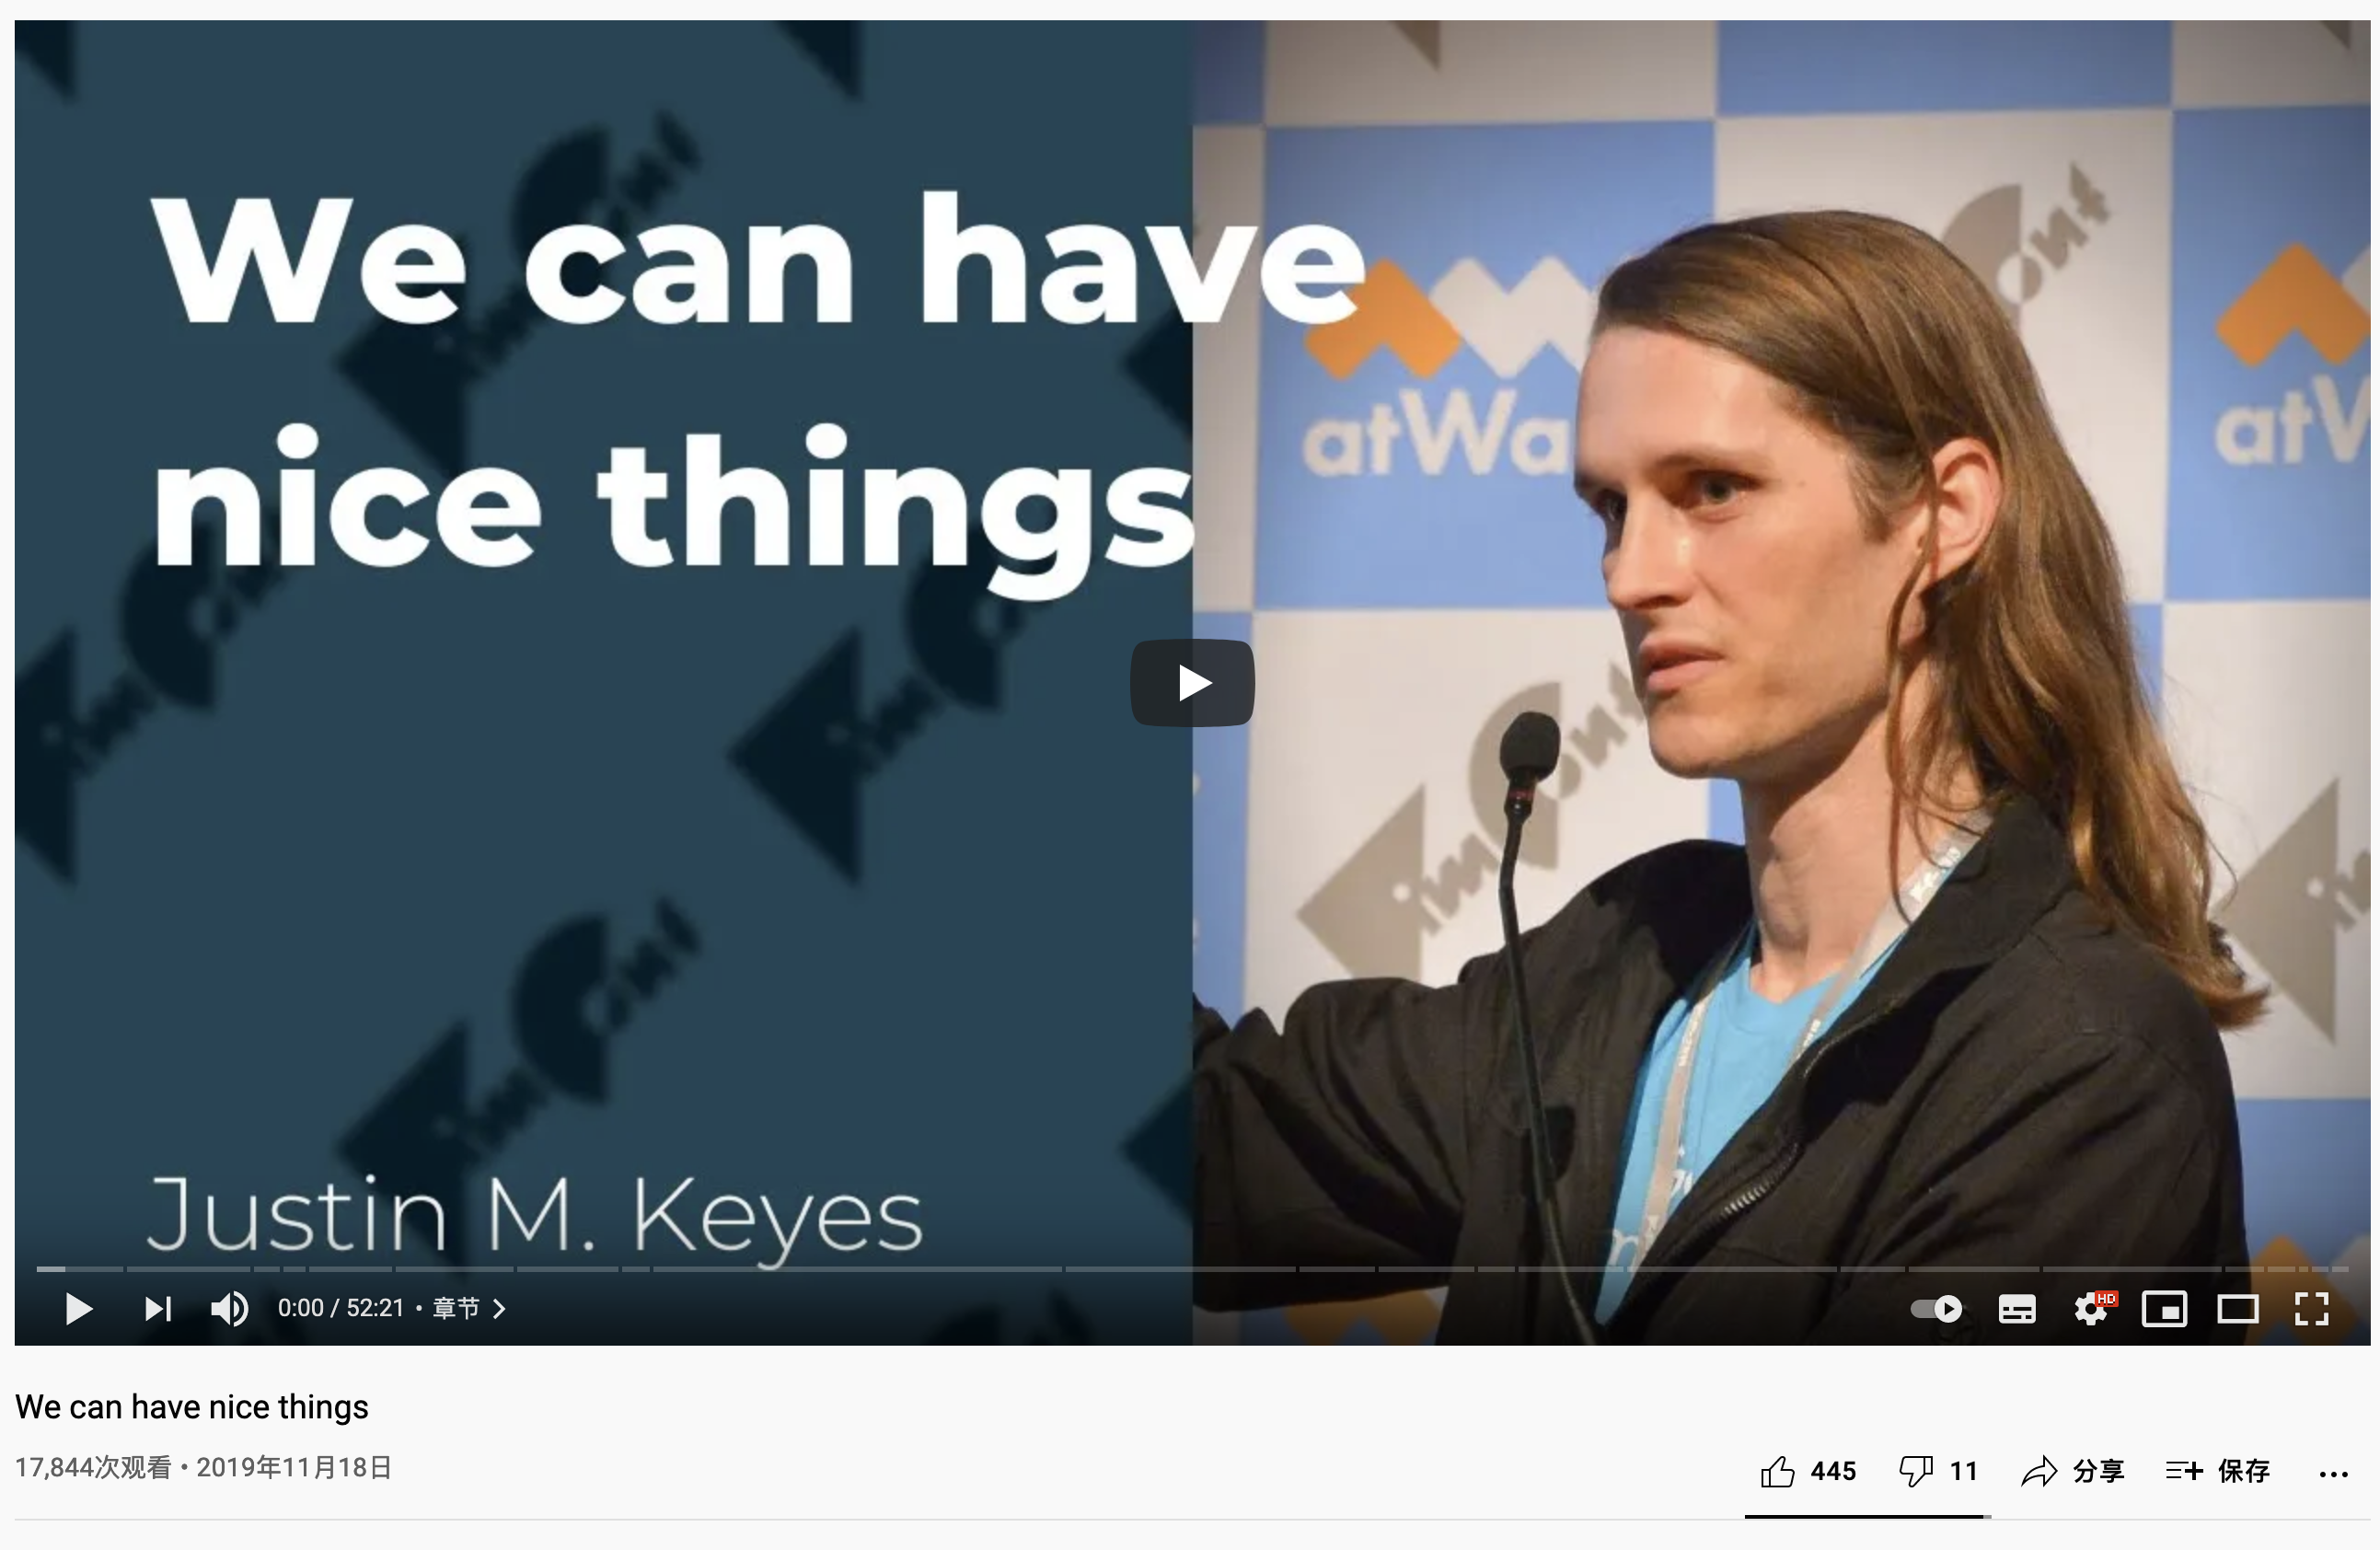
\includegraphics[width=\textwidth]{we_can_have_nice}

\end{frame}


\begin{frame}{Why Nvim?}

	I wanted to replace emacs

	\vspace{1em}

	
\includegraphics[width=\textwidth]{home_page}

	\vspace{1em}

	...and make CLI as easy as VSCode

\end{frame}


\begin{frame}{Vim "philosophy"}

	\begin{itemize}

		\begin{multicols}{2}

			\item unix-y

			\item ad hoc

			\item macro driven

			\item minimalist

			\item extensible

			\item composible

			\item conservative

		\end{multicols}

	\end{itemize}

	\rule{\textwidth}{0.1em}

	\textbf{But at what cost?}

	\begin{itemize}

		\begin{multicols}{2}

			\item slowiness

			\item jankiness

			\item ossification

			\item interlocking

			\item beginner hostile

			\item dx hostile

		\end{multicols}

	\end{itemize}


\end{frame}


\begin{frame}{Terraforming Nvim}
	
	\begin{block}{Terraforming}

		\vspace{0.5em}

		Making nvim more hospitable for developers

		\vspace{0.5em}

	\end{block}

	\rule{\textwidth}{0.1em}

	\begin{itemize}

		\begin{multicols}{2}

			\item lua
			
			\item vim.api.nvim\_*

			\item API clients

			\item tree-sitter

			\item libuv

			\item extmarks

			\item virtual text

			\item remote UI

		\end{multicols}

	\end{itemize}

	... and more 

\end{frame}


\begin{frame}{Novelty Tolerance}

	Beyond just the API, but also the \textbf{culture too}

	\rule{\textwidth}{0.1em}

	Follow the leader

\end{frame}


\begin{frame}{What Programmers Like}

	\textbf{Structure \& Regularity}

	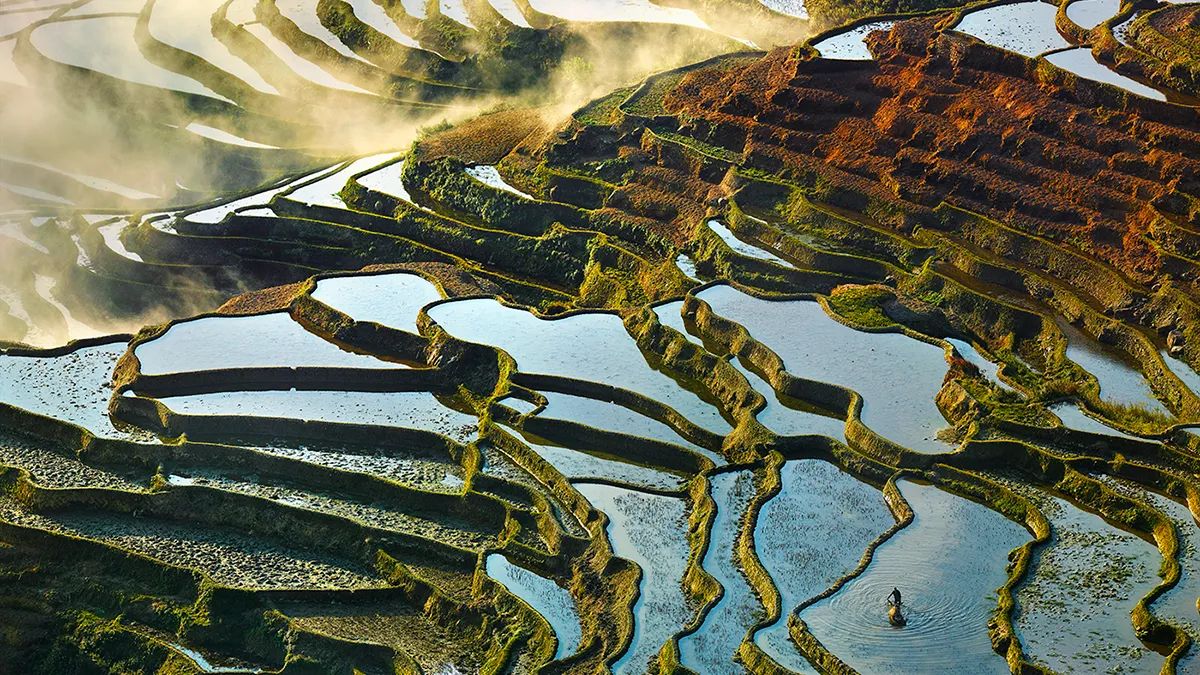
\includegraphics[width=\textwidth]{rice_paddy}

	\textit{thousand year old rice paddy}

\end{frame}


\begin{frame}{Structurizing}


	% \begin{itemize}

	% 	\item Vimscript the hardway

	% 	      % lxz : why not lua?

	% 	\item Library enabling async await in lua (Structured Concurrency)

	% 	      % https://github.com/ms-jpq/lua-async-await

	% 	\item CHADTree (Structured rendering)

	% 	      % https://github.com/ms-jpq/chadtree

	% 	\item coq.nvim (Structured plugins)

	% 	      % https://github.com/ms-jpq/coq_nvim

	% \end{itemize}


	% \begin{enumerate}

	% 	\item Shove things into registers

	% 	\item Invoke key sequences

	% 	\item Esoteric regexes

	% 	\item Footguns

	% 	      % Case sensitive == -> worse than JS

	% \end{enumerate}

	Libuv (same as in node) -> super powerful

	% Too hard to use in lua?

	\begin{enumerate}

		\item Callback hell

		\item Coroutines "too hard" to use

	\end{enumerate}

	% Don't spend too much time on this, it's 

	So I wrote \textit{async await} as a library

	% Same idea as clojure core.async

\end{frame}



\begin{frame}{CHADTree: Notable Features}


	\begin{enumerate}

		\item Feature 1

		\item Feature 2

		\item Feature 3

	\end{enumerate}


\end{frame}


\begin{frame}{coq.nvim: Notable Features}


	\begin{enumerate}

		\item Feature 1

		\item Feature 2

		\item Feature 3

	\end{enumerate}


\end{frame}


\begin{frame}{coq.nvim: Notable Features}


	\begin{enumerate}

		\item Feature 1

		\item Feature 2

		\item Feature 3

	\end{enumerate}


\end{frame}



\begin{frame}{CHADTree Observations}


	\begin{enumerate}

		\item File system walking is very fast

		\item Rendering is slow

		\item Extensible filemanagers are the slowest

	\end{enumerate}


\end{frame}


\begin{frame}{CHADTree Solutions}


	\begin{enumerate}

		\item Do the opposite of UNIX "philosophy"

		      % Pull other plugins into CHADTree, instead of the other way around

		\item AOT compile other plugins into CHADTree

		\item React

		      % Wrote a 70 line typesafe React before, it's on my Github

	\end{enumerate}


\end{frame}



\begin{frame}{Virtual Rendering Engine}


	Two stage rendering

	Virtual rendering target

	\begin{enumerate}

		\item Compute designed state


		\item Compute linewise hash of desired state

	\end{enumerate}


	Actual rendering target

	\begin{enumerate}

		\item Fetch hash -> compute minimal diff


		\item Apply patch onto buffers, store hash


	\end{enumerate}


	Side effect: can now perform (almost) transactional retries


	% Lua is a very nice lang, but doing this is just too hard
	% Transpilers do not seem super mature

\end{frame}



\begin{frame}{Going in the opposite direction}

	Need to support third party plugins, but...

	Notice a pattern here:

	\begin{enumerate}

		\item nvim-completion-manager -> ncm2

		\item neocomplete.vim -> deoplete.nvim -> ddc.vim

		\item nvim-compe -> nvim-cmp

		\item completion-nvim :: still ok!

		\item YouCompleteMe :: still ok!

		\item coc :: going great!

	\end{enumerate}


\end{frame}


\begin{frame}{The protocols of Nvim}

	Protocols are meant to be ossified

	Implementations are not

	Some protocols inherent to Nvim

	\begin{enumerate}

		\item vim.bo.omnifunc

		\item :h complete-items

		\item vim.lsp.protocol

	\end{enumerate}

\end{frame}


\begin{frame}[standout]

	questions, comments, stuff

	hola@bigly.dog

\end{frame}


\end{document}
